% !TeX root = ../main.tex

\chapter{Theoretical Background} \label{chap:2}
\section{Working principle of AWG}\label{sec:2.1}
    \lipsum
    \begin{align}
        \upDelta \lambda_\text{FSR} &= N_\text{ch} \upDelta \lambda\text{,}\label{eq:awg-DFSRLamFSR}\\
        m' &= \frac{\lambda_0}{\upDelta \lambda_\text{FSR}}\text{,}\label{eq:awg-m'}\\
        m &= \text{round}\left(m' \frac{n_{\text{eff}_0}}{N_\ur{\text{g}}}\right)\text{,}\label{eq:awg-m}\\
        N_\text{g} &= n_{\text{eff}_0} - \lambda \frac{\mathrm{d}n_{\text{eff}_0}}{\mathrm{d}\lambda}\text{,}\label{eq:awg-Na}\\
        \upDelta L_\text{0} &= m \frac{\lambda_0}{n_{\text{eff}_0}}\text{,}\label{eq:awg-dL}\\
        f& = R_\text{o} = 2\,R_\text{i} = \frac{n_\text{s}d D}{m' \upDelta \lambda}\text{,}\label{eq:awg-Ro}\\
        D_\text{FSR} &= D\,N_\text{ch}\text{,}\label{eq:awg-DFSR}
    \end{align}
    /lipsum

\section{Working principle of thermal tuning} \label{sec:2.2}
    To date, some thermally tunable AWG leveraging the relation between heat and material refractive indices are implemented on different platforms 
    \cite{TTAWG-p1, TTAWG-p2, TTAWG-p3, TTAWG-n1, TTAWG-n2, TBDTAWG}. 
    Normally, a thermo-optic coefficient of 1.68$\cdot$10\SP{-4}~/K is utilized for silicon layer.
    For more accurate evaluation, two-dimensional (2-D) simulations are performed using the heat transportation 
    followed by the finite-difference eigenmode (FDE) solver 
    to obtain the thermal-diffusion as well as the refractive index change profiles at different electrical voltages. 

\section{Working principle of BGACDC} \label{sec:2.3}
    Recently, 
    a mechanism based on Bragg grating-assisted contra-directional coupling have been used to achieve a flat-top filtering response for CWDM system. 
    To demonstrate the working principle of the device, 
    two concepts including perturbed-permittivity coupled-mode theory (PPCMT) and its anytical expression for brief evaluation of resulting spectrum 
    are geiven in the following two subsections.

\subsection{Coupled-mode theory for permittivity perturbation} \label{sec:2.3.1}
    The differential equations for \ur{Bragg grating-assisted contra-directional coupling} are minimally adjusted 
    based on the perturbed-permittivity coupled-mode theory for fiber Bragg grating presented in \cite{kashyap-fbg}, 
    and given in the following
    \begin{align}
        \frac{\partial B_\text{\textit{\textmu}}}{\partial z} &= j\kappa_\text{dc,\textit{\textmu \textmu}}B_\text{\textit{\textmu}} + 
                j\kappa_\text{ac,\textit{v\textmu}}A_\text{\textit{v}}\cdot \textit{e}^{-j(\upDelta \beta z - \phi (z))}\text{,}\label{eqCMT:1} \\
        \frac{\partial A_\text{\textit{v}}}{\partial z} &= -j\kappa_\text{dc,\ur{\textit{vv}}}A_\text{\textit{v}} - 
                j\kappa_\text{ac,\textit{\textmu v}}B_\text{\textit{\textmu}}
                \cdot \textit{e}^{j(\upDelta \beta z - \phi (z))}\text{,}\label{eqCMT:2}\\
        \kappa_\text{dc,(\textit{vv,\textmu \textmu})} &= \frac{\omega \varepsilon_0}{4} \iint \upDelta \varepsilon_\text{r,dc} (x,y)
            \textbf{E}_\text{\textit{v,\textmu}}(x,y)
            \cdot \textbf{E}_\text{\textit{v,\textmu}}^\text{*}(x,y)\text{d}x\text{d}y\text{,}\label{eqCMT:3} \\
        \kappa_\text{ac,(\textit{v\textmu,\textmu v})} &= \frac{\omega \varepsilon_0}{4} \iint \upDelta \varepsilon_\text{r,ac} (x,y)
            \textbf{E}_\text{\textit{v,\textmu}}(x,y)
            \cdot \textbf{E}_\text{\textit{\textmu ,v}}^\text{*}(x,y)\text{d}x\text{d}y\text{,}\label{eqCMT:4}
    \end{align}
    \lipsum
    
\subsection{Transfer matrix \ur{method}} \label{sec:2.3.2}
    To decribe the contra-directional coupling behavior more clearly with mathematical expression, 
    a transfer matrix in terms of eigenvalue $\alpha_\text{ei}$ is derived as 
    \begin{align}
        \begin{bmatrix}
            R(z) \\
            S(z)
        \end{bmatrix} &= 
        \begin{bmatrix}
            T_\text{11}(z) & T_\text{12}(z) \\
            T_\text{21}(z) & T_\text{22}(z)
        \end{bmatrix}
        \begin{bmatrix}
            R(0) \\
            S(0)
        \end{bmatrix}\text{,}\label{eqCMT:5}\\
        T_\text{11(22)}(z) &= \text{cosh}(\alpha z){\substack{-\\(+)}} j\frac{\delta}{\alpha}\text{sinh}(\alpha z)\text{,}\label{eqCMT:6}\\
        T_\text{12(21)}(z) &= {\substack{-\\(+)}} j\frac{\kappa_\text{ac,\textit{\textmu v}(\textit{v\textmu})}}
        {\alpha}\text{sinh}(\alpha z)\text{,}\label{eqCMT:7}\\
        \delta &= \frac{1}{2}(\kappa_\text{dc,\textit{vv}} + 
                \kappa_\text{dc,\textit{\textmu \textmu}} + \upDelta \beta)\text{,}\label{eqCMT:8}\\
        \upDelta \beta &= \beta_\text{\textit{v}} + \beta_\text{\textit{\textmu}} - \frac{2\pi N}{\Lambda}\text{,}\label{eqCMT:9}\\
        \left|\frac{S(0)}{R(0)}\right|_{S(L)=0}^2 &= \left|\frac{-j\frac{\kappa_\text{ac,\textit{v\textmu}}}{\alpha}\text{sinh}(\alpha L)}
                {\text{cosh}(\alpha L)+j\frac{\delta}{\alpha}\text{sinh}(\alpha L)}\right|^2\text{.}\label{eqCMT:10}
    \end{align}
    \lipsum

\section{Simulation methods} \label{sec:2.4}
    In this section, four solvers/methods are briefly introduced to efficiently design the devices presented in the latter chapters. 
    To evaluate feasibility of a TTAWG, 
    the beam propagation method (BPM), heat transport solver, and FDE solver respectively provided by 
    RSoft and Lumerical are utilized. 
    On the other hand, 
    FDE and finite-difference time-domain (FDTD) are employed to obtain the reflected filtering response of a Bragg grating-assisted structure. 

\subsection{Beam propagation method (BPM)} \label{sec:2.4.1}
    The main concept of BPM \cite{oka-book-bpm} relies on the assumption of dividing electric field $E(x,y,z)$ into two terms including 
    the axially slowly warying envelope term $\phi(x,y,z)$ and the rapid varying phase term exp($-jkn_{0}z$), 
    where $E(x,y,z)$ satisfies the three-dimensional (3-D) scalar wave equation (Helmholtz equation) expressed by 
    \begin{equation}
        \frac{\partial ^2 E}{\partial x^2} + \frac{\partial ^2 E}{\partial y^2} + \frac{\partial ^2 E}{\partial z^2} + 
            k^2 n^2 (x,y,z) E = 0\text{,}\label{eq:Helmholtz}
    \end{equation}
    with the electric field $E(x,y,z)$ equivalent to $\phi(x,y,z)\cdot \text{exp}(-jkn_\text{0}z)$. 
    By the substitution of $E$ into (\ref{eq:Helmholtz}), 
    a formula for BPM can be obtained as 
    \begin{equation}
        \nabla_\text{T}^2 - j2kn_{0}\frac{\partial \phi}{\partial z} + k^2 (n^2 - n_0^2)\phi = 0\text{,}\label{eq:bpm}
    \end{equation}
    where $\nabla_\text{T}^2$ is an operator expressed as 
    \begin{equation}
        \nabla_\text{T}^2 = \frac{\partial^2}{\partial x^2} + \frac{\partial^2}{\partial y^2}\text{.}\label{eq:operator}
    \end{equation}
    To obtain the spatial derivative envelop along the propagation direction, 
    (\ref{eq:bpm}) is utilzied and derived into 
    \begin{equation}
        \frac{\partial \phi}{\partial z} = \frac{-j}{2kn_{\text{EIM}_0}^{}}\frac{\partial^2 \phi}{\partial x^2} - 
            \frac{-jk}{2n_{\text{EIM}_0}^{}}\left[n_\text{EIM}^2 (x,z) - n_{\text{EIM}_0}^2\right]\phi\text{,}\label{eq:bpmz}
    \end{equation}
    where the effective indices $n_{\text{EIM}_0}^{}$ and $n_\text{EIM}^{}$ 
    are the effective indices calculated using effective index method (EIM) 
    to include simulation information within height ($y$) direction. 
    In Chapter~\ref{chap:3}, the BPM provided by RSoft 
    is employed for efficient analysis of the diffractive field as well as beam focusing behavior 
    within the region of two FPRs at different operating wavelengths. 

\subsection{Heat Transport (HT) solver} \label{sec:2.4.2}
    To evaluate heat transport behavior in terms of external electrical sources, 
    three electrical-related equations should be concerened firstly, including 
    (a) the electrical current equation (Ohm's law), 
    (b) the auxiliary continuity equation, and 
    (c) Gauss' law for DC permittivity $\varepsilon$, which can be respectively obtained by 
    \begin{align}
        \textbf{J} = \sigma \textbf{E} = -\sigma \nabla V\text{,}\label{eq:HT1}\\
        \frac{\partial \rho}{\partial t} = -\nabla\cdot\textbf{J}\text{,}\label{eq:HT2}\\
        -\nabla\cdot(\varepsilon \nabla V) = \rho \text{,}\label{eq:HT3}
    \end{align}
    where \textbf{J}, \textbf{E}, $\sigma$, $V$, $\rho$, and $t$ denote 
    current density vector, electrical field vector, electrical conductivity, electrical potential, charge density, and time, respectively. 
    For homogeneous material system, 
    a differential equation can thus be derived into 
    \begin{equation}
        \frac{\partial \rho}{\partial t} + \frac{\sigma}{\varepsilon}\rho = 0\textit{.}\label{eq:HT4}
    \end{equation}
    Under the assumption of quasi-static approximation or steady-state, 
    (\ref{eq:HT1}) combined with (\ref{eq:HT2}) can then reduces into 
    \begin{equation}
        \nabla\cdot(\sigma\textbf{E}) = 0\text{.}\label{eq:HT5}
    \end{equation}
    On the other hand, 
    a $\sigma$-related equation, \textit{i.e.}, 
    power dissipation due to Ohimic loss, can be described by 
    \begin{equation}
        P = \textbf{J}\cdot\textbf{E} = \sigma E^2\text{,}\label{eq:HT6}
    \end{equation}
    and applied to the heat transport equation as a heat energy transfer rate $Q = P$. 
    While Q can be obtained by 
    \begin{equation}
        Q = m_\text{d} C_\text{p} \frac{\partial T}{\partial t} - \nabla \cdot (k_\text{c}\nabla T)\text{,}\label{eq:HT7}
    \end{equation}
    where $m_\text{d}$, $C_\text{p}$, $T$, $t$, and $k_\text{c}$ represent 
    the mass density, the specific heat, temperature, time, and the thermal conductivity, respectively.
    By solving the last three equations (\ref{eq:HT5})--(\ref{eq:HT7}), 
    the heat transportation behavior can be evaluated. 
    In this dissertation, 
    the heat transport (HT) solver provided by Lumerical is utilized to efficiently analyze the thermal tuning problem. 
    % Considering that the thermal-tuning function of TTAWG is introduced by external electrical voltages, 
    % an analysis of heat distributions at different voltages is carried out using heat transport (HT) solver (Lumerical Inc.). 
    % The temperature distributions within a solid medium can be solved over the heat transport equation expressed as 
    % \begin{equation}
        % m_\text{d} C_\text{p} \frac{\partial T}{\partial t} - \nabla \cdot (k_\text{c}\nabla T) = Q\text{,}\label{eq:HT}
    % \end{equation}
    % where $m_\text{d}$, $C_\text{p}$, $k_\text{c}$, and $Q$ represent the mass density, the specific heat, the thermal conductivity, 
    % and the applied heat energy transfer rate, respectively. 
    % Within a homogeneous material region, a differential equation is derived as 
    % \begin{equation}
        % \frac{\partial \rho}{\partial t} + \frac{\sigma \rho}{\varepsilon} = 0\text{,}\label{eq:HTsc}
    % \end{equation}
    % for self-consistent condition with (\ref{eq:HT}).
    % Given that the solution to (\ref{eq:HTsc}) is an exponential decay with a relaxation time $\tau = \varepsilon / \sigma$, 
    % the quasi-static approximation of $\partial \rho / \partial t \sim 0$ can be valid for the time scales of $t \gg \tau$. 
    % In addition, by applying the approximation, 
    % the continuity equation can be reduced into $\nabla\cdot(\sigma \textbf{E}) = \text{0}$.
    % In steady-state with the solution condition $\partial T / \partial t = \text{0}$, 
    % the heat transport equation can be further reduced into 
    % \begin{equation}
        % -\nabla\cdot(k\nabla T) = Q\text{,}\label{eq:HTss}
    % \end{equation}
    % with the electric current equation, again, becoming 
    % \begin{equation}
        % \nabla\cdot(\sigma \textbf{E}) = 0\text{.}\label{eq:HTce}
    % \end{equation}
    % By applying the steady-state HT equation with appropriate finite-element mesh as well as boundary conditions offered by the HT solver, 
    % one can easily evaluate the heat distribution over the modeled region. 
    
\subsection{Finite-difference eigenmode (FDE) solver} \label{sec:2.4.3}
    To solve eigenmode more efficiently, 
    the commercial finite-difference eigenmode (FDE) solver provided by Lumerical is utilized in the following two chapters. 
    During the simulations, 
    the FD algorithm is employed to mesh the waveguide geometry. 
    Maxwell's equations are then formulated into a matrix eigenvalue problem
    which is solved by using sparse matrix technique \cite{lu-fde, fde-oe}. 

\subsection{Finite-difference time-domain (FDTD) solver} \label{sec:2.4.4}
    FDTD, blah, blah, blah, blah, blah, blah, blah, blah, blah, blah, blah, blah, 
    \begin{align}
        \frac{\partial\textbf{B}}{\partial t} &= -\nabla\times\textbf{E} - \textbf{M}\text{,}\label{eq:ME1}\\
        \frac{\partial\textbf{D}}{\partial t} &= \nabla\times\textbf{H}-\textbf{J}\text{,}\label{eq:ME2}\\
        \nabla\cdot\textbf{D} &= \text{0}\text{,}\label{eq:ME3}\\
        \nabla\cdot\textbf{B} &= \text{0}\text{,}\label{eq:ME4}
    \end{align}
    blah, blah, blah, blah, blah, blah, blah, blah, blah, blah, blah, blah, blah, blah, blah, blah, blah, 
    blah, blah, blah, blah, blah, blah, blah, blah, blah, blah, blah, blah, blah, blah, blah, blah, blah, 
    blah, blah, blah, blah, blah, blah, blah, blah, blah, blah, blah, blah, blah, blah, blah, blah, blah, 
    blah, blah, blah, blah, blah, blah, blah, blah, blah, blah, blah, blah, blah, blah, blah, blah, blah, 
    \begin{equation}
        \textbf{J} = \textbf{J}_\text{source}+\sigma \textbf{E};\;\;\;\;
        \textbf{M} = \textbf{M}_\text{source}+\sigma^* \textbf{H}\text{,}\label{eq:JM}
    \end{equation}
    where $\sigma$ and $\sigma^*$ denote electric conductivity and equivalent magnetic loss, respectively, 
    under the condition of linear, isotropic, and nondispersive materials, which can be illustrated by 
    \begin{equation}
        \textbf{D} = \varepsilon\textbf{E} = \varepsilon_\text{r}\varepsilon_\text{0} \textbf{E}\text{;} \;
        \textbf{B} = \mu\textbf{H} = \mu_\text{r}\mu_\text{0}\textbf{H}\text{,}\label{eq:DB}
    \end{equation}
    with $\varepsilon$, $\varepsilon_\text{r}$, $\varepsilon_0$, $\mu$, $\mu_\text{r}$, and $\mu_0$ representing 
    electrical permittivity, relative permittivity, free-space permittivity, 
    magnetic permeability, relative permeability, and free-space permeability, respectively. 
    By the substitution of (\ref{eq:JM}, \ref{eq:DB}) into (\ref{eq:ME1}, \ref{eq:ME2}), 
    two Maxwell's curl equations in linear, isotropic, nondispersive, and lossy materials can be derived as 
    \begin{equation}
        \frac{\partial\textbf{H}}{\partial t} = -\frac{1}{\mu}\nabla\times\textbf{E} - 
            \frac{1}{\mu}\left(\textbf{M}_\text{source}+\sigma^* \textbf{H}\right)\text{;}\;
        \frac{\partial\textbf{E}}{\partial t} = \frac{1}{\varepsilon}\nabla\times\textbf{H} - 
            \frac{1}{\varepsilon}\left(\textbf{J}_\text{source}+\sigma\textbf{E}\right)\text{,}\label{eq:MEfdtdcurl2}
    \end{equation}
    and then six vector components in Cartesian coordinates can be obtained \cite{taflove-book-fdtd} as 
    % \begin{align}
        % \stags
        % \frac{\partial H_x}{\partial t} &= \frac{-1}{\mu}\left[
            % \frac{\partial E_z}{\partial y} - \frac{\partial E_y}{\partial z} + (M_{\text{source}_x}+\sigma^* H_x)
            % \right]\text{,}\tag{\stag}\label{eq:fdtdHx}\\
        % \frac{\partial H_y}{\partial t} &= \frac{-1}{\mu}\left[
            % \frac{\partial E_x}{\partial z} - \frac{\partial E_z}{\partial x} + (M_{\text{source}_y}+\sigma^* H_y)
            % \right]\text{,}\tag{\stag}\label{eq:fdtdHy}\\
        % \frac{\partial H_z}{\partial t} &= \frac{-1}{\mu}\left[
            % \frac{\partial E_y}{\partial x} - \frac{\partial E_x}{\partial y} + (M_{\text{source}_z}+\sigma^* H_z)
            % \right]\text{,}\tag{\stag}\label{eq:fdtdHz}\\
        % \stags
        % \frac{\partial E_x}{\partial t} &= \frac{1}{\varepsilon}\left[
            % \frac{\partial H_z}{\partial y} - \frac{\partial H_y}{\partial z} - (J_{\text{source}_x}+\sigma E_x)
            % \right]\text{,}\tag{\stag}\label{eq:fdtdEx}\\
        % \frac{\partial E_y}{\partial t} &= \frac{1}{\varepsilon}\left[
            % \frac{\partial H_x}{\partial z} - \frac{\partial H_z}{\partial x} - (J_{\text{source}_y}+\sigma E_y)
            % \right]\text{,}\tag{\stag}\label{eq:fdtdEy}\\
        % \frac{\partial E_z}{\partial t} &= \frac{1}{\varepsilon}\left[
            % \frac{\partial H_y}{\partial x} - \frac{\partial H_x}{\partial y} - (J_{\text{source}_z}+\sigma E_z)
            % \right]\text{.}\tag{\stag}\label{eq:fdtdEz}
    % \end{align}
    \begin{align}
        \frac{\partial H_x}{\partial t} = \frac{-1}{\mu}\left[
            \frac{\partial E_z}{\partial y} - \frac{\partial E_y}{\partial z} + (M_{\text{source}_x}+\sigma^* H_x)
            \right]\text{,}
        \frac{\partial E_x}{\partial t} = \frac{1}{\varepsilon}\left[
            \frac{\partial H_z}{\partial y} - \frac{\partial H_y}{\partial z} - (J_{\text{source}_x}+\sigma E_x)
            \right]\text{,}\label{eq:fdtdHx}\\
        \frac{\partial H_y}{\partial t} = \frac{-1}{\mu}\left[
            \frac{\partial E_x}{\partial z} - \frac{\partial E_z}{\partial x} + (M_{\text{source}_y}+\sigma^* H_y)
            \right]\text{,}
        \frac{\partial E_y}{\partial t} = \frac{1}{\varepsilon}\left[
            \frac{\partial H_x}{\partial z} - \frac{\partial H_z}{\partial x} - (J_{\text{source}_y}+\sigma E_y)
            \right]\text{,}\label{eq:fdtdHy}\\
        \frac{\partial H_z}{\partial t} = \frac{-1}{\mu}\left[
            \frac{\partial E_y}{\partial x} - \frac{\partial E_x}{\partial y} + (M_{\text{source}_z}+\sigma^* H_z)
            \right]\text{,}
        \frac{\partial E_z}{\partial t} = \frac{1}{\varepsilon}\left[
            \frac{\partial H_y}{\partial x} - \frac{\partial H_x}{\partial y} - (J_{\text{source}_z}+\sigma E_z)
            \right]\text{.}\label{eq:fdtdHz}
    \end{align}
    
    \begin{figure}[htp]
		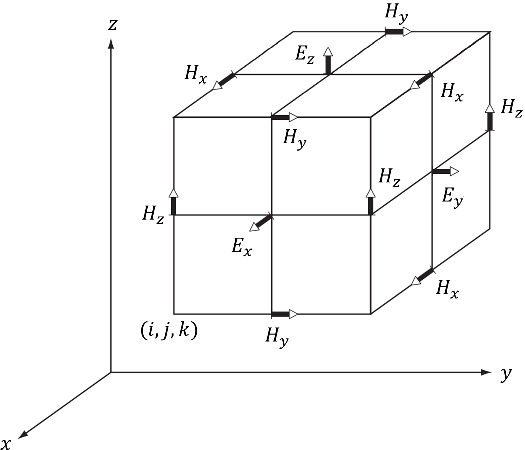
\includegraphics{/YeeCell/YeeCell_300dpi.pdf}
		\centering
		\caption{\label{fig:YeeCell}Yee's Cell for solving time- and space-dependent electric and magnetic fields.}
	\end{figure}
    \clearpage
    \lipsum
    \begin{align}
        \stags
        \begin{split}
            \left. H_x \right\rvert_{i,j+\frac{1}{2},k+\frac{1}{2}}^{n+1} = 
            \left. H_x \right\rvert_{i,j+\frac{1}{2},k+\frac{1}{2}}^{n} 
                &- \frac{\upDelta t}{\mu\upDelta y}
                    \left(\left. E_z\right\rvert_{i,j+1,k+1}^{n+\frac{1}{2}} - 
                        \left. E_z\right\rvert_{i,j,k+1}^{n+\frac{1}{2}}\right) \\
                &+ \frac{\upDelta t}{\mu\upDelta z}
                    \left(\left. E_y\right\rvert_{i,j+\frac{1}{2},k+1}^{n+\frac{1}{2}} - 
                        \left. E_y\right\rvert_{i,j+\frac{1}{2},k}^{n+\frac{1}{2}}\right)\text{,}
        \end{split}\tag{\stag}\label{eq:fdtdgridHx}\\
        \begin{split}
            \left. H_y \right\rvert_{i+\frac{1}{2},j,k+\frac{1}{2}}^{n+1} = 
            \left. H_y \right\rvert_{i+\frac{1}{2},j,k+\frac{1}{2}}^{n} 
                &-\frac{\upDelta t}{\mu\upDelta z}
                    \left(\left. E_x\right\rvert_{i+\frac{1}{2},j,k+1}^{n+\frac{1}{2}} - 
                        \left. E_x\right\rvert_{i+\frac{1}{2},j,k}^{n+\frac{1}{2}}\right) \\
                &+\frac{\upDelta t}{\mu\upDelta x}
                    \left(\left. E_z\right\rvert_{i+1,j,k+\frac{1}{2}}^{n+\frac{1}{2}} - 
                        \left. E_z\right\rvert_{i+1,j,k+\frac{1}{2}}^{n+\frac{1}{2}}\right)\text{,}
        \end{split}\tag{\stag}\label{eq:fdtdgridHy}\\
        \begin{split}
            \left. H_z \right\rvert_{i+\frac{1}{2},j+\frac{1}{2},k}^{n+1} = 
            \left. H_z \right\rvert_{i+\frac{1}{2},j+\frac{1}{2},k}^{n} 
                &-\frac{\upDelta t}{\mu\upDelta x}
                    \left(\left. E_y\right\rvert_{i+1,j+\frac{1}{2},k}^{n+\frac{1}{2}} - 
                        \left. E_y\right\rvert_{i+1,j+\frac{1}{2},k}^{n+\frac{1}{2}}\right) \\
                &+\frac{\upDelta t}{\mu\upDelta y}
                    \left(\left. E_x\right\rvert_{i+\frac{1}{2},j+1,k}^{n+\frac{1}{2}} - 
                        \left. E_x\right\rvert_{i+\frac{1}{2},j+1,k}^{n+\frac{1}{2}}\right)\text{,}
        \end{split}\tag{\stag}\label{eq:fdtdgridHz}\\
        \stags
        \begin{split}
            \left. E_x \right\rvert_{i+\frac{1}{2},j,k}^{n+\frac{1}{2}} = 
            \left. E_x \right\rvert_{i+\frac{1}{2},j,k}^{n-\frac{1}{2}} 
                &+\frac{\upDelta t}{\varepsilon\upDelta y}
                    \left(\left. H_z\right\rvert_{i+\frac{1}{2},j+\frac{1}{2},k}^{n} - 
                        \left. H_z\right\rvert_{i+\frac{1}{2},j-\frac{1}{2},k}^{n}\right) \\
                &-\frac{\upDelta t}{\varepsilon\upDelta z}
                    \left(\left. H_y\right\rvert_{i+\frac{1}{2},j,k+\frac{1}{2}}^{n} - 
                        \left. H_y\right\rvert_{i+\frac{1}{2},j,k-\frac{1}{2}}^{n}\right)\text{,}
        \end{split}\tag{\stag}\label{eq:fdtdgridEx}\\
        \begin{split}
            \left. E_y \right\rvert_{i,j+\frac{1}{2},k}^{n+\frac{1}{2}} = 
            \left. E_y \right\rvert_{i,j+\frac{1}{2},k}^{n-\frac{1}{2}} 
                &+\frac{\upDelta t}{\varepsilon\upDelta z}
                    \left(\left. H_x\right\rvert_{i,j+\frac{1}{2},k+\frac{1}{2}}^{n} - 
                        \left. H_x\right\rvert_{i,j+\frac{1}{2},k-\frac{1}{2}}^{n}\right) \\
                &-\frac{\upDelta t}{\varepsilon\upDelta x}
                    \left(\left. H_z\right\rvert_{i+\frac{1}{2},j+\frac{1}{2},k}^{n} - 
                        \left. H_z\right\rvert_{i-\frac{1}{2},j+\frac{1}{2},k}^{n}\right)\text{,}
        \end{split}\tag{\stag}\label{eq:fdtdgridEy}\\
        \begin{split}
            \left. E_z \right\rvert_{i,j,k+\frac{1}{2}}^{n+\frac{1}{2}} = 
            \left. E_z \right\rvert_{i,j,k+\frac{1}{2}}^{n-\frac{1}{2}} 
                &+\frac{\upDelta t}{\varepsilon\upDelta x}
                    \left(\left. H_y\right\rvert_{i+\frac{1}{2},j,k+\frac{1}{2}}^{n} - 
                        \left. H_y\right\rvert_{i-\frac{1}{2},j,k+\frac{1}{2}}^{n}\right) \\
                &-\frac{\upDelta t}{\varepsilon\upDelta y}
                    \left(\left. H_x\right\rvert_{i,j+\frac{1}{2},k+\frac{1}{2}}^{n} - 
                        \left. H_x\right\rvert_{i,j\frac{1}{2},k+\frac{1}{2}}^{n}\right)\text{.}
        \end{split}\tag{\stag}\label{eq:fdtdgridEz}
    \end{align}
    \clearpage
    In summary, the power coupling behavior between electric and magnetic fields 
    obtained from Maxwell's equations over space and time domain can be described within Yee's cell. 
    By using the central differences for the space derivatives and the leapfrog scheme for the time derivatives, 
    six components ($E_x, E_y, E_z, H_x, H_y, H_z$) of both fields at the specific spatial and 
    the temporal grid can be utilized to evaluate 
    the components at the next grid. 
    In this dissertation, 
    the FDTD solver provided by Lumerical \cite{lu-fdtd} is utilized 
    for efficient analysis as well as the visualization of the 3-D electric and magnetic fields. 
    